%!TEX root = ../../tcc.tex

\section{Engenharia de Software}

O Transmission é um programa bastante complexo e grande. Por exemplo, todos os arquivos
que são usados na versão GTK+ somam pouco mais de 86 mil linhas. Desenvolvido por cinco
programadores em nove anos, possui versões de vários tipos e sistemas operacionais. Um
programa desse porte poderia usar conhecimentos de Engenharia de Software para questões
de manutenção de código, melhoria da qualidade de desenvolvimento, enfim, todos os
aspectos da produção do programa. Alguns desses aspectos são notáveis pelos seus
recursos, entre eles o site, fórum de usuários, código do programa, etc.

\begin{description}
    \item[modularização:] o Transmission possui o código organizado de forma que a
        funcionalidade está separada e independente da implementação da interface
        gráfica (\emph{front end}). Isso permite que o programa funcione da mesma forma
        para todas as versões desenvolvidas, já que possui o mesmo núcleo de
        funcionamento (\emph{back end}).

    \begin{figure}[H]
        \centering
        \fbox{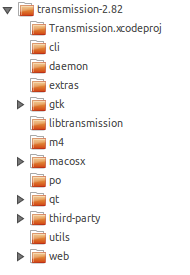
\includegraphics[width=.33\textwidth]{pastas.png}}
        \caption{estruturas de pastas do Transmission}
        \label{fig:pastas}
    \end{figure}

        As implementações visuais do Transmission utilizam os \emph{frameworks}
        GTK+ \cite{site:gtk}, Qt \cite{site:qt} e ncurses \cite{site:ncurses}, além do
        modo de linha de comando;

    \item[multiplataforma:] tendo seu código modularizado, basta uma ferramenta que
        saiba compilá-lo de acordo com as ferramentas que o computador possui. Para
        isso, utiliza as ferramentas: Autoconf \cite{site:autoconf}, que gera os arquivos de
        configuração da compilação, dependendo do sistema operacional e dos softwares
        básicos instalados; e Automake \cite{site:automake}, que gera o arquivo de
        compilação utilizando o de configuração gerado pelo Autoconf;

    \item[comentários de código:] boa parte do código do Transmission não possui
        comentários, o que muitas vezes dificultou o entendimento de seu funcionamento;

    \item[testes unitários:] são códigos que executam verificações da corretude de uma
        parte específica de código, geralmente no nível de funções. Existem alguns
        testes unitários escritos, mas não para toda implementação de funcionalidade.
        Por exemplo, o código de leitura e decodificação de \gls{magnetlink};
\end{description}

\cfile[label="./libtransmission/metainfo-test.c"]{./Codes/chap4/023-metainfo-test.c}

\begin{description}
    \item[internacionalização:] de forma semelhante ao que é feito atualmente com
        o desenvolvimento de aplicativos para celulares, o Transmission é desenvolvido
        com seus textos escritos em arquivos externos, um para cada linguagem,
        facilitando o processo de tradução do programa;

    \item[código aberto e livre:] o código do Transmission é acessível a todos, podendo
        ser portado a outras plataformas. Além disso, qualquer um pode participar do seu
        desenvolvimento, bastando entrar em contato com os atuais programadores.
\end{description}